% fdps_sc15.tex
% paper about FDPS for SC 15
% Author: A. Tanikawa
% 1 March 2015

\documentclass{acm_proc_article-sp}
%%%%%%%%%%%%%%%%%%%%%%%%%%%%%%%%%%%%%%%%%%%%%%%%%%%%%%%%%%%%%%%%
\usepackage{listings}
\usepackage{color}
\newcommand{\myvec}[1]{\vec{#1}}
\newcommand{\redtext}[1]{\textcolor{red}{#1}}
\newcommand{\araa}{Annual Review of Astronomy and Astrophysics}
\newcommand{\icarus}{Icarus}
\newcommand{\mnras}{Monthly Notices of the Royal Astronomical Society}
\newcommand{\apj}{Astrophysical Journal}
\newcommand{\pasa}{Publications of the Astronomical Society of Australia}
\newcommand{\pasj}{Publications of the Astronomical Society of Japan}
\newcommand{\aap}{Astronomy and Astrophysics}
%%%%%%%%%%%%%%%%%%%%%%%%%%%%%%%%%%%%%%%%%%%%%%%%%%%%%%%%%%%%%%%%

\begin{document}

\title{FDPS: A Novel Framework for Developing High-Performance
  Particle Simulation Codes for Distributed-Memory Systems}

%\subtitle{}

\numberofauthors{5}

\author{
  \alignauthor
  Masaki Iwasawa \\
  \affaddr{RIKEN Advanced Institute for Computational Science} \\
  \affaddr{7--1--26, Minatojima-minami-machi, Chuo-ku, Kobe, Hyogo, Japan} \\
  \email{masaki.iwasawa@riken.jp}
  %
  \alignauthor
  Ataru Tanikawa \\
  \affaddr{RIKEN Advanced Institute for Computational Science} \\
  \affaddr{7--1--26, Minatojima-minami-machi, Chuo-ku, Kobe, Hyogo, Japan} \\
  \email{ataru.tanikawa@riken.jp}
  %
  \alignauthor
  Natsuki Hosono \\
  \affaddr{RIKEN Advanced Institute for Computational Science} \\
  \affaddr{7--1--26, Minatojima-minami-machi, Chuo-ku, Kobe, Hyogo, Japan} \\
  \email{natsuki.hosono@riken.jp}
  \and
  %
  \alignauthor
  Keigo Nitadori \\
  \affaddr{RIKEN Advanced Institute for Computational Science} \\
  \affaddr{7--1--26, Minatojima-minami-machi, Chuo-ku, Kobe, Hyogo, Japan} \\
  \email{keigo@riken.jp}
  %
  \alignauthor
  Takayuki Muranushi \\
  \affaddr{RIKEN Advanced Institute for Computational Science} \\
  \affaddr{7--1--26, Minatojima-minami-machi, Chuo-ku, Kobe, Hyogo, Japan} \\
  \email{takayuki.muranushi@riken.jp}
  %
  \alignauthor
  Junichiro Makino \\
  \affaddr{RIKEN Advanced Institute for Computational Science} \\
  \affaddr{7--1--26, Minatojima-minami-machi, Chuo-ku, Kobe, Hyogo, Japan} \\
  \email{jmakino@riken.jp}
}

\maketitle

\begin{abstract}

  We have developed FDPS (Framework for Developing Particle
  Simulator), which enables researchers and programmers to develop
  high-performance particle simulation codes easily.  The basic idea
  of FDPS is to separate the program code for complex parallelization
  including domain decomposition, redistribution of particles, and
  exchange of particle information for interaction calculation between
  nodes, from actual interaction calculation and orbital
  integration. FDPS provides the former part and the users write the
  latter. Thus, a user can implement a high-performance $N$-body code
  only in 120 lines. In this paper, we present the structure and
  implementation of FDPS, and describe its performance on two sample
  applications: gravitational $N$-body simulation and Smoothed
  Particle Hydrodynamics simulation. Both codes show very good
  parallel efficiency and scalability on the K computer. FDPS lets the
  researchers concentrate on the implementation of physics and
  mathematical schemes, without wasting their time on the development
  and performance tuning of their codes.

\end{abstract}

\category{D.1.3}{Software}{PROGRAMMING TECHNIQUES}[Concurrent
  Programming]
%%
\category{I.6.7}{Computing Methodologies}{SIMULATION AND
  MODELING}[Simulation Support Systems]
%%
\category{J.2}{Computer Applications}{PHYSICAL SCIENCES AND
  ENGINEERING}[Astronomy]
%%
\category{J.2}{Computer Applications}{PHYSICAL SCIENCES AND
  ENGINEERING}[Earth and atmospheric sciences]
%%
\terms{Algorithm, Performance}
%%
\keywords{Framework for implementing parallel codes, high-performance
  computing, particle simulation}

\section{Introduction}

In the field of computational astronomy, simulations based on particle
methods have been widely used. In such simulations, a system is either
physically a collection of particles as in the case of star clusters,
galaxies and dark-matter halos, or modeled by a collection of
particles, as in SPH (smoothed particle hydrodynamics) simulation of
astrophysical fluids.  Since particles move automatically as the
result of integration of the equation of motion of the particle,
particle-based simulations have an advantage for systems experiencing
strong deformation or systems with high density contrast.  This is one
of the reasons why particle-based simulations are widely used in
astronomy. Examples of particle-based simulations include cosmological
simulations or planet-formation simulations with gravitational
$N$-body code, simulations of star and galaxy formation with the SPH
code or other particle-based codes, and simulations of planetesimal
formation with the DEM (discrete element method) code.

We need to use a large number of particles to improve the resolution
and accuracy of particle-based simulations, and in order to do so we
need to increase the calculation speed and need to use
distributed-memory parallel machines efficiently. In other words, we
need to implement efficient algorithms such as the Barnes-Hut tree
algorithm \citep{1986Natur.324..446B}, the TreePM
algorithm \citep{1995ApJS...98..355X} or the Fast Multipole Method
\citep{2000ApJ...536L..39D} to distributed-memory parallel computers.
In order to achieve high efficiency, we need to divide a computational
domain into subdomains in such a way that minimizes the need of
communication between processors to maintain the division and to
perform interaction calculations. To be more specific, parallel
implementations of particle-based simulations contain the following
three procedures to achieve the high efficiency: (a) domain
decomposition, in which the subdomains to be assigned to computing
nodes are determined so that the calculation times are balanced, (b)
particle exchange, in which particles are moved to computing nodes
corresponding to the subdomains to which they belong, and (c)
interaction information exchange, in which each computing node
collects the information necessary to calculate the interactions on
its particles.  In addition, we need to make use of multiple CPU cores
in one processor chip and SIMD (single instruction multiple data)
execution units in one CPU core, or in some cases GPGPUs
(general-purpose computing on graphics processing units) or other
accelerators.


%% In order to improve the resolution and accuracy of particle-based
%% simulations, it is necessary to utilize present-day HPC systems.
%% However, to develop a calculation code for particle systems which can
%% achieve high efficiency on present-day HPC systems is difficult and
%% time-consuming. There are several reasons for this difficulty. In
%% order to achieve high efficiency, we need to decompose the
%% computational domain, assign subdomains to computing nodes, and
%% redistribute particles according to their positions. This
%% decomposition should be dynamically changed to guarantee the good load
%% balance. This division of the computational domain means that
%% computing nodes need to exchange the information of particles to
%% evaluate the interactions on their particles. To achieve high
%% efficiency, the amount of the exchanged data must be minimized, and
%% interaction calculation should also be efficient, making good use of
%% cache memory and SIMD execution units. It is also important to make
%% use of GPGPUs or other types of accelerators, if available.

In the case of gravitational $N$-body problems, there are a number of
works in which the efficient parallelization is
discussed \citep{1994JCoPh.111..136S, 1996NewA....1..133D,
2004PASJ...56..521M, 2009PASJ...61.1319I,
Ishiyama:2012:PAN:2388996.2389003}.  The use of SIMD units is
discussed in \citet{2006NewA...12..169N}, \citet{2012NewA...17...82T}
and \citet{2013NewA...19...74T}, and GPGPUs
in \citet{2009NewA...14..630G}, \citet{hamada2009novel}, \citet{Hamada:2009:THN:1654059.1654123}, \citet{Hamada:2010:TAN:1884643.1884644}, \citet{2012JCoPh.231.2825B}
and
\citet{Bedorf:2014:PGT:2683593.2683600}.

In the field of molecular dynamics, several groups have been working
on parallel implementations. Examples of such efforts include
Amber \citep{2015AMBER}, CHARMM \citep{2009CHARMM},
Desmond \citep{GB14}, GROMACS \citep{2014GROMACS},
LAMMPS \citep{1995LAMMPS}, NAMD \citep{2005NAMD}. In the field of CFD
(computational fluid dynamics), Many commercial and non-commercial
packages now support SPH or other particle-based methods
(PAM-CRASH \footnote{https://www.esi-group.com/pam-crash},
LS-DYNA \footnote{http://www.lstc.com/products/ls-dyna},
Adventure/LexADV \footnote{http://adventure.sys.t.u-tokyo.ac.jp/lexadv})


Currently, parallel application codes are being developed for each of
specific applications of particle methods. Each of these codes
requires multi-year effort of a multi-person team. We believe this
situation is problematic because of the following reasons.

First, it has become difficult for researchers to try a new method or
just a new experiment which requires even a small modification of
existing large codes. If one wants to test a new numerical scheme, the
first thing he or she would do is to write a small program and to do
simple tests. This can be easily done, as far as that program runs on
one processor. However, if he or she then wants to try a
production-level large calculation using the new method, the
parallelization for distributed-memory machines is necessary, and
other optimizations are also necessary. However, to develop such a
program in a reasonable time is impossible for a single person, or
even for a team, unless they already have experiences of developing
such a code.

Second, even for a team of people developing a parallel code for one
specific problem, it has become difficult to take care of all the
optimizations necessary to achieve a reasonable efficiency on recent
processors. In fact, the efficiency of many simulation codes mentioned
above on today's latest microprocessors are rather poor, simply
because the development team does not have enough time and expertise
to implement necessary optimizations (in some case they require the
change of data structure, control structure and algorithms).

In our opinion, these difficulties have significantly slowed down
researchs in the numerical methods and also the research using
large-scale simulations.

%% Thus, to develop a code which has all of these necessary features for
%% present-day HPC systems has become a big project which requires
%% multi-year effort of a multi-person team. It has become difficult for
%% researchers outside such a team to try any new experiments which
%% requires nontrivial modification of the code. If one wants to develop
%% a new numerical scheme for particle-based simulation or to apply it to
%% new problem, it is necessary to write his/her own code. However, it is
%% practically impossible for a single person, or even for a group of
%% people, to develop a new code which can run efficiently on present-day
%% HPC systems in a reasonable time.  This difficulty, in our opinion,
%% has slowed down the evolution of the entire field of computational
%% science for the last two decades. Here we discussed the situation of
%% particle-based codes. The situation of grid-based codes is similar.

%% JM --- modified up to here as of Feb 8 0:46

We have developed FDPS (Framework for Developing Particle
Simulator)\footnote{https://github.com/FDPS/FDPS} \citep{2015FDPS} in
order to solve these difficulties. The goal of FDPS is to let
researchers concentrate on the implementation of numerical schemes and
physics, without spending too much time on parallelization and code
optimization. To achieve this goal, we separate a code into domain
decomposition, particle exchange, interaction information exchange and
fast interaction calculation using Barnes-Hut tree algorithm and/or
neighbor search and the rest of the code. We implement these functions
as ``template'' libraries in C++ language. The reason why we use the
template libraries is to allow the researchers to define their own
data structure for particles and their own functions for
particle-particle interactions, and to provide them with
highly-optimized libraries with small software overhead.  A user of
FDPS needs to define the data structure and the function to evaluate
particle-particle interaction. Using them as template arguments, FDPS
effectively generates the highly-optimized library functions which
perform complex operations listed above.

From users' point of view, what is necessary is to write the program
in C++, using FDPS library functions and to compile it using a
standard C++ compiler. Using FDPS, users thus can write their
particle-based simulation codes for gravitational $N$-body problem,
SPH, MD (molecular dynamics), DEM, or many other particle-based
methods, without spending their time on parallelization and complex
optimization. The compiled code will run efficiently on large-scale
parallel machines.

For grid-based or FEM (Finite Element Method) applications, there are
many frameworks for developing parallel applications. For example,
Cactus \citep{2003Cactus} has been widely used for numerical
relativity, and BoxLib \footnote{https://ccse.lbl.gov/BoxLib/} is
designed for AMR (adaptive mesh refinement). For particle-based
simulations, such frameworks have not been widely used yet, though
there were early efforts as in \citet{1995CoPhC..87..266W}, which is
limited to long-range, $1/r$ potential. More recently, LexADV\_EMPS is
currently being developed \citep{2015LexADV_EMPS}. As its name
suggests, it is rather specialized to the EMPS (Explicit Moving
Particle Simulation) method \citep{2014Murotani}.




In section~\ref{sec:user}, we describe the basic design concept of
FDPS.  In section~\ref{sec:implementation}, we describe the
implementation of parallel algorithms in FDPS. In
section~\ref{sec:performance}, we present the measured performance for
three astrophysical applications developed using FDPS. In
section~\ref{sec:performancemodel}, we construct a performance model
and predict the performance of FDPS on near-future supercomputers.
Finally, we summarize this study in section~\ref{sec:conclusion}.

%Some contents in sections \ref{sec:user}, \ref{sec:implementation} and
%4.1 have been published in \citet{2015FDPS}.

%In section~\ref{sec:performance}, we illustrate
%how FDPS actually simplifies the development of user programs, using
%three sample FDPS applications, and describe their performance. 

% LocalWords:  HPC subdomains SIMD GPGPUs multi FDPS parallelized SPH
% LocalWords:  parallelization


\section{How FDPS works}
\label{sec:user}

In this section, we describe how FDPS works in detail.  In
section~\ref{sec:design}, we describe the design concept of FDPS. In
section~\ref{sec:samplecode}, we present an $N$-body simulation code
as an example, and describe how FDPS does the parallelization and what
a user program should do.

\subsection{Design concept}
\label{sec:design}

In this section, we present the basic design concept of FDPS. We first
present the abstract view of calculation codes for particle-based
simulations on distributed-memory parallel computers, and then
describe how such abstraction is realized in FDPS.


\subsubsection{Abstract view of particle-based simulation codes}
\label{sec:view}

In a particle-based simulation code that uses the space decomposition on
distributed-memory parallel computers, the calculation proceeds in the
following steps:
\begin{enumerate}

\item The computational domain is divided into subdomains, and each
  subdomain is assigned to one MPI process. This step is usually
  called domain decomposition. Here, minimization of inter-process
  communication and a good load balance among  processes should be
  achieved.
 \label{proc:decompose}

\item Particles are exchanged among  processes, so that each
  process owns particles in its subdomain. In this paper we call this
  step particle exchange.
  \label{proc:exchange}

\item Each process collects the information necessary to calculate the
  interactions on its particles. We call this step
  interaction-information exchange.
  \label{proc:interactionexchange}

\item Each process calculates interactions between particles in its
  subdomain. We call this step interaction calculation.
  \label{proc:interaction}

\item The data for each particle are updated using the calculated
  interactions. This part is done without inter-process communication.
   \label{proc:local}
\end{enumerate}

Steps \ref{proc:decompose}, \ref{proc:exchange}, and
\ref{proc:interactionexchange} involve parallelization and
inter-process communications. FDPS provides library functions to
perform these parts. Therefore, users of FDPS do not have to write the
parallelization and/or inter-process communication part of their own
code at all.

Step \ref{proc:interaction} does not involve inter-process
communication. However, this step are necessary to perform the actual
calculation of interactions between two particles.  Users of FDPS
should write a simple interaction kernel. The actual interaction
calculation using the tree algorithm or neighbor search is done in the
FDPS side.

%However, it requires either the use of tree algorithm
%or FMM (long-range interactions), or neighbor search (short-range
%interactions), and actual calculation of interactions between
%particles.  Users of FDPS should write a simple interaction kernel,
%and actual interaction calculation using the tree algorithm or
%neighbor search is done in the FDPS side.

Step \ref{proc:local} involves neither inter-process communication nor
interaction calculation. Users of FDPS should and can write their own
program for this part. 

%In the following we describe briefly how FDPS provide the application
%program interface (API) for steps \ref{proc:decompose} through.  for
%arbitrary systems of particles.

%% JM 2016081418

FDPS can be used to implement particle-based simulation codes for
initial value problems which can be expressed as the following
ordinary differential equations:

\begin{eqnarray}
%\begin{align}
  \frac{d\myvec{u}_i}{dt} = \myvec{g}\left(\sum_j^N \myvec{f}
  (\myvec{u}_i, \myvec{u}_j), \myvec{u}_i\right). \label{eq:geq}
%\end{align}
\end{eqnarray}
  
Here, $N$ is the number of particles in the system, $\myvec{u}_i$ is
a vector which represents the physical quantities of  particle $i$, 
$\myvec{f}$ is a function which describes
the contribution of particle $j$ to the time derivative of
physical quantities of particle $i$, and $\myvec{g}$ is a function
which converts the sum of the contributions to the actual time
derivative. In the case of gravitational $N$-body
simulation, $\myvec{u}_i$ contains position, velocity, mass, and other
parameters of  particle $i$, $\myvec{f}$ is the gravitational force
from particle $j$ to particle $i$, and 
$\myvec{g}$ gives velocity as the time derivative of  position and
calculated acceleration as the time derivative of velocity.

Hereafter, we call a particle that receives the interaction
``$i$-particle'', and a particle exerting that interaction
``$j$-particle''. The actual contents of vector $\myvec{u}_i$ and the
functional forms of $\myvec{f}$ and $\myvec{g}$ depend on the physical
system and numerical scheme used.

In equation (\ref{eq:geq}) we included only the pairwise interactions,
because usually the calculation cost of the pairwise interaction is
the highest even when many-body interaction is important. For example,
angle and torsion of bonding force in simulation of organic molecules
can be done in the user code, with small additional computing cost.


\subsubsection{Design concept of FDPS}
\label{sec:concept}

In this section, we describe how the abstract view presented in the
previous section is actually expressed in the FDPS API (application
programming interface).  The API of FDPS is defined as a set of
template library functions in C++ language.


\begin{figure}
  \begin{center}
    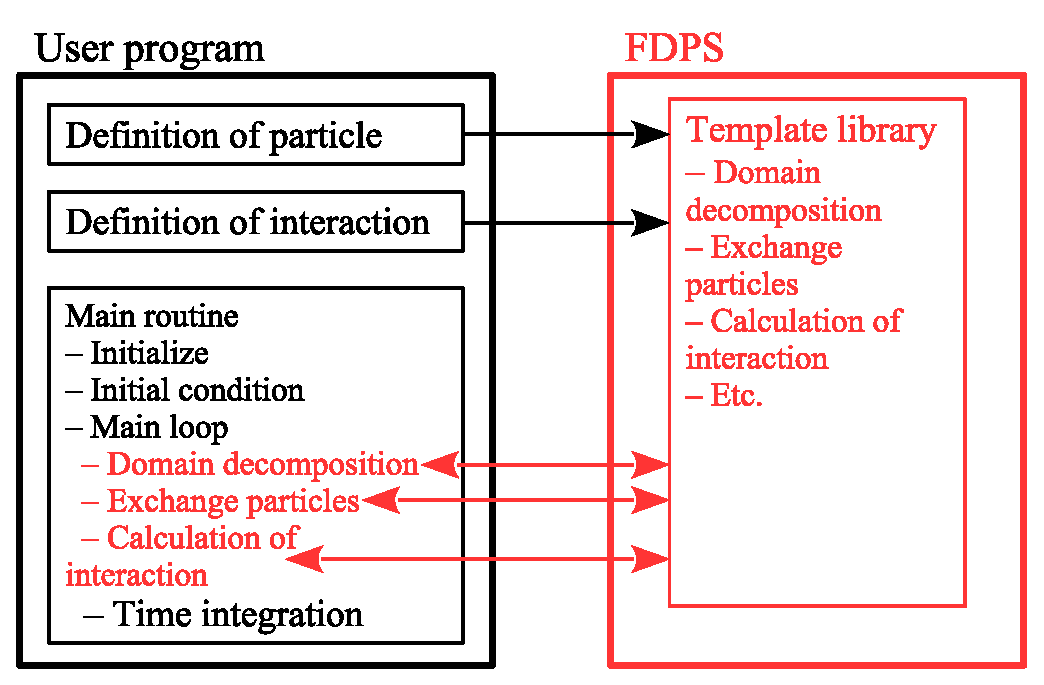
\includegraphics[width=8cm]{figure/concept.eps}
  \end{center}
  \caption{The basic concept of FDPS. The user program gives the
    definitions of particle and interaction to FDPS, and calls FDPS
    APIs.}
  \label{fig:concept}
\end{figure}


Figure~\ref{fig:concept} shows how a user program and FDPS library
functions interact.  The user program gives the definition of a
particle $\myvec{u}_i$ and particle-particle interaction $\myvec{f}$
to FDPS at the compile time. They are written in the standard C++
language. Thus, the user program [at least the main() function]
currently should be written in C++\footnote{We will investigate a
  possible way to use APIs of FDPS from programs written in Fortran.}.

%% 02081511

The user program first does the initialization of FDPS library. When
the user program is compiled for the MPI environment, the
initialization of MPI communication is done in the FDPS initialization
function.  The setup of the initial condition is done in the user
program.  It is possible to use file input function defined in FDPS.
In the main integration loop, domain decomposition, particle exchange,
interaction information exchange and force calculation are all done
through library calls to FDPS.  The time integration of the physical
quantities of particles using the calculated interaction, is done
within the user program.

%% A user of FDPS can develop the simulation code in the following three
%% steps:
%% \begin{enumerate}
%% \item Define the data structure for $\myvec{u}_i$, as a class in the
%%   C++ language.
%% \item Define the function $\myvec{f}$. It receives arrays of
%%   $i$-particles and $j$-particles, and calculates and accumulates
%%   $\myvec{f}$ on $i$-particles.

%%   %It should be a function object in C++ language\footnote{A function
%%   %pointer of C language can be operable.}, which receives arrays of
%%   %  $i$-particles and $j$-particles, and calculates and accumulates
%%   %  $\myvec{f}$ on $i$-particles.
  
%% \item Write the user program using the data class and functions
%%   provided by FDPS. Currently, the user program should also be written
%%   in C++.
%% \end{enumerate}

Note that it is possible to implement multi-stage integration schemes
such as the Runge-Kutta schemes using FDPS. FDPS can evaluate the
right-hand side of equation (\ref{eq:geq}) for a given set of
$\myvec{u}_i$. Therefore, the derivative calculation for intermediate
steps can be done by passing $\myvec{u}_i$ containing appropriate
values.

The parallelization using MPI is completely taken care by FDPS, and
the use of OpenMP is also taken care by FDPS for the interaction
calculation. In order to achieve high performance, the interaction
calculation should make efficient use of the cache memory and SIMD
units. In FDPS, this is done by requiring an interaction calculation
function to calculate the interactions between multiple $i$- and
$j$-particles. In this way, the amount of memory access is
significantly reduced, since single $j$-particle is used to calculate
the interaction on multiple $i$-particles ($i$-particles are also in
the cache memory). To make the efficient use of the SIMD execution
units, currently the user should write the interaction calculation
loop so that the compiler can generate SIMD instructions. Of course,
the use of libraries optimized for specific architectures
\citep{2006NewA...12..169N, 2012NewA...17...82T, 2013NewA...19...74T}
would guarantee very high performance.

It is also possible to use GPUs and other accelerators for the
interaction calculation. In order to reduce the communication
overhead, so-called ``multiwalk'' method \citet{hamada2009novel}, is
implemented. Thus, interaction calculation kernels for accelerators
should take multiple sets of the pair of $i$- and $j$-particles. The
performance of this version will be discussed elsewhere.

\begin{figure}
  \begin{center}
    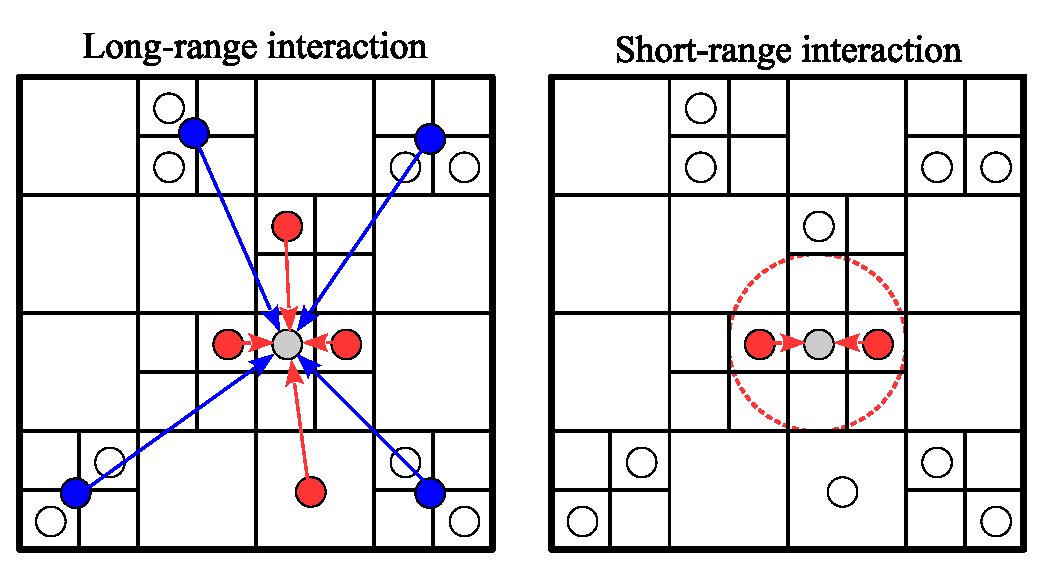
\includegraphics[width=8cm]{figure/force_type.eps}
  \end{center}
  \caption{Long-range interaction (left) and short-range interaction
    (right). Gray, red, and blue points are $i$-particles,
    $j$-particles, and superparticles, respectively.}
  \label{fig:forcetype}
\end{figure}

As stated earlier, FDPS performs the neighbor search if the interaction
is of short-range nature. If the long-range interaction is used,
currently FDPS uses the Barnes-Hut tree algorithm. In other words,
within FDPS, the distinction between the long-range and short-range
interactions is not a physical one but an operational one. If we want
to apply the treecode, it is a long-range interaction. Otherwise, it is
a short-range interaction.  Thus, we can use the simple tree
algorithm for pure $1/r$ gravity and the TreePM scheme
\citep{1995ApJS...98..355X, 2000ApJS..128..561B, 2002JApA...23..185B,
  2004NewA....9..111D, 2005MNRAS.364.1105S, 2005PASJ...57..849Y,
  2009PASJ...61.1319I, Ishiyama:2012:PAN:2388996.2389003} for the
periodic boundary.


Figure~\ref{fig:forcetype} illustrates the long-range and short-range
interactions and how they are calculated in FDPS.

For  long-range interactions, Barnes-Hut algorithm is used. Thus, the
interactions from a group of distant particles are replaced by that of
a superparticle, and  equation~(\ref{eq:geq}) is modified to 
%\begin{align}
\begin{eqnarray}
  \frac{d\myvec{u}_i}{dt} = \myvec{g}\left( \sum_j^{N_{\mathrm{J},i}}
  \myvec{f}(\myvec{u}_i,\myvec{u}_j) + \sum_{j'}^{N_{\mathrm{S},i}}
  \myvec{f'}(\myvec{u}_i,\myvec{u'}_{j'}), \myvec{u}_i
  \right), \label{eq:geqL}
%\end{align}
\end{eqnarray}
where $N_{\mathrm{J},i}$ and $N_{\mathrm{S},i}$ are, the number of
$j$-particles and superparticles for which we apply multipole-like
expansion, the vector $\myvec{u'}_{j'}$ is the physical quantity
vector of a superparticle, and the function $\myvec{f'}$ indicates the
interaction exerted on particle $i$ by the superparticle $j'$. In
simulations with a large number of particles $N$, $N_{\mathrm{J},i}$
and $N_{\mathrm{S},i}$ are many orders of magnitude smaller than $N$.
A user need to give functions to construct superparticles from
particles and to calculate the interaction from superparticles. Since
the most common use of the long-range interaction is for $1/r$
potential, FDPS includes standard implementation of these functions
for $1/r$ potential for  up to the quadrupole moment.




% LocalWords:  FDPS subdomains subdomain MPI parallelization dt discretized API
% LocalWords:  APIs timestep Runge Kutta OpenMP SIMD vectorization AoS SoA PME
% LocalWords:  multipole FFT TreePM parallelized superparticles superparticle
% LocalWords:  quadrupole


\subsection{A working example --- gravitational \secit{N}-body problem}
\label{sec:samplecode}

In this section, we present a complete user code for the gravitational
$N$-body problem with the open boundary condition, to illustrate how a
user write an application program using FDPS.  The gravitational
interaction is handled as ``long-range'' type in FDPS. Therefore, we
need to provide the data type and interaction calculation functions
for superparticles. In order to keep the sample code short, we use the
center-of-mass approximation and use the same data class and
interaction function for real particles and superparticles.


For the gravitational
$N$-body problem, the physical quantity vector $\myvec{u}_i$ and interaction functions
$\myvec{f}$, $\myvec{f'}$, and $\myvec{g}$ are given by:
%\begin{align}
\begin{eqnarray}
  \myvec{u}_i &=& (\myvec{r}_i,
  \myvec{v}_i,m_i), \label{eq:PhysicalVectorNbody} \\
%%  
  \myvec{f} (\myvec{u}_i, \myvec{u}_j) &=& \frac{Gm_j \left(
    \myvec{r}_j - \myvec{r}_i \right)}{ \left( |\myvec{r}_j -
    \myvec{r}_i|^2 + \epsilon_i^2
    \right)^{3/2}}, \label{eq:ParticleParticleNbody} \\
%%
  \myvec{f'} (\myvec{u}_i, \myvec{u'}_j) &=& \frac{Gm_j' \left(
    \myvec{r}_j - \myvec{r'}_i \right)}{ \left( |\myvec{r}_j -
    \myvec{r'}_i|^2 + \epsilon_i^2
    \right)^{3/2}}, \label{eq:ParticleSuperparticleNbody} \\
%%
  \myvec{g}(\myvec{F},\myvec{u}_i)  &=& (\myvec{v}_i,\myvec{F},0), \\
  \myvec{F} &=& \sum_j^{N_{\mathrm{J},i}}
  \myvec{f}(\myvec{u}_i,\myvec{u}_j) + \sum_{j'}^{N_{\mathrm{S},i}}
  \myvec{f'}(\myvec{u}_i,\myvec{u'}_{j'}), \myvec{u}_i,
\label{eq:ConversionNbody}
%\end{align}
\end{eqnarray}
where $m_i$, $\myvec{r}_i$, $\myvec{v}_i$, and $\epsilon_i$ are, the
mass, position, velocity, and gravitational softening of particle $i$,
$m_j'$ and $\myvec{r'}_j$ are, the mass and position of a
superparticle $j$, and $G$ is the gravitational constant.  Note that
the shapes of the functions $\myvec{f}$ and $\myvec{f'}$ are the same.

Listing~\ref{code:samplecode} shows the complete code which can be
compiled and run, not only on a single-core machine but also
massively-parallel, distributed-memory machines such as the  K
computer. The total number of lines is 117.


%\begin{lstlisting}[label=code:samplecode,numbers=left,numbersep=5pt,frame=single,basicstyle=\ttfamily,caption=A sample code of $N$-body simulation]
%\begin{lstlisting}[label=code:samplecode]
%\begin{lstlisting}[label=code:samplecode,numbers=left,numbersep=5pt,frame=single,basicstyle=\ttfamily,caption=A sample code of $N$-body simulation]
\begin{lstlisting}[label=code:samplecode,numbers=left,numbersep=5pt,frame=single,basicstyle=\ttfamily]
#include <particle_simulator.hpp>
using namespace PS;

class Nbody{
public:
    F64    mass, eps;
    F64vec pos, vel, acc;
    F64vec getPos() const {return pos;}
    F64 getCharge() const {return mass;}
    void copyFromFP(const Nbody &in){ 
        mass = in.mass;
        pos  = in.pos;
        eps  = in.eps;
    }
    void copyFromForce(const Nbody &out) {
        acc = out.acc;
    }    
    void clear() {
        acc = 0.0;
    }
    void readAscii(FILE *fp) {
        fscanf(fp,
               "%lf%lf%lf%lf%lf%lf%lf%lf",
               &mass, &eps,
               &pos.x, &pos.y, &pos.z,
               &vel.x, &vel.y, &vel.z);
    }
    void predict(F64 dt) {
        vel += (0.5 * dt) * acc;
        pos += dt * vel;
    }
    void correct(F64 dt) {
        vel += (0.5 * dt) * acc;
    }
};

template<class TPJ>
struct CalcGrav{
    void operator () (const Nbody * ip,
                      const S32 ni,
                      const TPJ * jp,
                      const S32 nj,
                      Nbody * force) {
        for(S32 i=0; i<ni; i++){
            F64vec xi  = ip[i].pos;
            F64    ep2 = ip[i].eps
                * ip[i].eps;
            F64vec ai = 0.0;
            for(S32 j=0; j<nj;j++){
                F64vec xj = jp[j].pos;
                F64vec dr = xi - xj;
                F64 mj  = jp[j].mass;
                F64 dr2 = dr * dr + ep2;
                F64 dri = 1.0 / sqrt(dr2);                
                ai -= (dri * dri * dri
                       * mj) * dr;
            }
            force[i].acc += ai;
        }
    }
};

template<class Tpsys>
void predict(Tpsys &p,
             const F64 dt) {
    S32 n = p.getNumberOfParticleLocal();
    for(S32 i = 0; i < n; i++)
        p[i].predict(dt);
}

template<class Tpsys>
void correct(Tpsys &p,
             const F64 dt) {
    S32 n = p.getNumberOfParticleLocal();
    for(S32 i = 0; i < n; i++)
        p[i].correct(dt);
}

template<class TDI, class TPS, class TTFF>
void calcGravAllAndWriteBack(TDI &dinfo,
                             TPS &ptcl,
                             TTFF &tree) {
    dinfo.decomposeDomainAll(ptcl);
    ptcl.exchangeParticle(dinfo);    
    tree.calcForceAllAndWriteBack
        (CalcGrav<Nbody>(),
         CalcGrav<SPJMonopole>(),
         ptcl, dinfo);    
}

int main(int argc, char *argv[]) {
    PS::Initialize(argc, argv);                               
    F32 time  = 0.0;
    const F32 tend  = 10.0;
    const F32 dtime = 1.0 / 128.0;
    PS::DomainInfo dinfo;
    dinfo.initialize();
    PS::ParticleSystem<Nbody> ptcl;
    ptcl.initialize();
    PS::TreeForForceLong<Nbody, Nbody,
        Nbody>::Monopole grav;
    grav.initialize(0);
    ptcl.readParticleAscii(argv[1]);
    calcGravAllAndWriteBack(dinfo,
                            ptcl,
                            grav);
    while(time < tend) {
        predict(ptcl, dtime);        
        calcGravAllAndWriteBack(dinfo,
                                ptcl,
                                grav);
        correct(ptcl, dtime);        
        time += dtime;
    }
    PS::Finalize();
    return 0;
}
\end{lstlisting}


In the following we describe how this sample code works.  It consists
of four parts: the declaration to use FDPS (lines 1 and 2), the
definition of the particle (the vector $\myvec{u}_i$) (lines 4 to 35),
the definition of the gravitational force (the functions $\myvec{f}$
and $\myvec{f'}$) (lines 37 to 61), and the actual user program.  The
actual user program consists of a main routine and functions which
call library functions of FDPS (lines 63 to line 117). In the
following, we discuss each of them.



In order to use FDPS, the user program should
include the header file ``particle\_simulator.hpp''.
All functionalities of  the standard FDPS library are
implemented  as the header source library, since they are 
template libraries which need to receive particle class and
interaction functions.  FDPS data types and functions are in  the namespace
``PS''. In this sample program, we declare ``PS''  as the default
namespace to simplify the code. In this sample, however, we did not
omit ``PS'' for FDPS functions and class templates to show that they
come from FDPS.

FDPS defines several data types. \texttt{F32/F64} are data types of
32-bit and 64-bit floating points. \texttt{S32} is the data type of
32-bit signed integer.
\texttt{F64vec} is the class of a vector consisting of three 64-bit
floating points. This class provides several operators, such as the
addition, subtraction and the inner product indicated by ``$*$''.  It
is not necessary to use these data types in the user program, but some
of the functions the user should provide these data types for the
return value.


In the second part, the particle data type, ({\it i.e.} the vector
$\myvec{u}_i$) is defined as class \texttt{Nbody}. It has the
following member variables: \texttt{mass} ($m_i$), \texttt{eps}
($\epsilon_i$), \texttt{pos} ($\myvec{r}_i$), \texttt{vel}
($\myvec{v}_i$), and \texttt{acc} ($d\myvec{v}_i/dt$). Although the
member variable \texttt{acc} does not appear in
equation~(\ref{eq:PhysicalVectorNbody}) -- (\ref{eq:ConversionNbody}),
we need this variable to store the result of the gravitational force
calculation. A particle class for FDPS must provide public member
functions \texttt{getPos}, \texttt{copyFromFP},
\texttt{copyFromForce} and \texttt{clear} in these names, so that the internal functions
of FDPS can access the data within the particle class.  For the name
of the particle class itself and the names of the member variables, a
user can use whatever names allowed by the C++ syntax.  The member
functions \texttt{predict} and \texttt{correct} are used to integrate
the orbits of particles. These are not related to FDPS.  Since the
interaction is pure $1/r$ type, the construction method for
superparticles provided by FDPS can be used and they are not shown
here.

In the third part, the interaction functions $\myvec{f}$ and
$\myvec{f'}$ are defined. In this example, actually they are the same,
except for the class definition for $j$-particles. Therefore, this
argument is given as an argument with the template data
type \texttt{TPJ}, so that a single source code can be used to
generate two functions.  The interaction function used in FDPS should
have the following five arguments. The first argument \texttt{ip} is
the pointer to the array of $i$-particles which receive the
interaction. The second argument \texttt{ni} is the number of
$i$-particles. The third argument \texttt{jp} is the pointer to the
array of $j$-particles or superparticles which exert the
interaction. The fourth argument \texttt{nj} is the number of
$j$-particles or super-particles. The fifth argument \texttt{force} is
the pointer to the array of variables of a user-defined class to which
the calculated interactions on $i$-particles can be stored. In this
example, we used the particle class itself, but this can be another
class or a simple array.

In this example, the interaction function is a function object
declared as a \texttt{struct}, with the only member
function \texttt{operator ()}. FDPS can also accept a function pointer
for the interaction function, which would look a bit more familiar to
most readers.  In this example, the interaction is calculated through
a simple double loop. In order to achieve high efficiency, this part
should be replaced by a code optimized for specific architectures. In
other words, a user needs to optimize just this single function to
achieve very high efficiency.


In the fourth part, the main routine and user-defined functions are
defined.  In the following, we describe the main routine in detail,
and briefly discuss other functions. The main routine consists of the
following seven steps:
\begin{enumerate}
\item Initialize FDPS (line 92). \label{proc:init}
\item Set simulation time and timestep (lines 93 to 95). \label{proc:literal}
\item Create and initialize objects of FDPS classes (lines 96 to 102). \label{proc:construct}
\item Read in particle data from a file (line 103). \label{proc:input}
\item Calculate the gravitational forces on all the particles at the
  initial time (lines 104 to 106). \label{proc:calcinteraction}
\item Integrate the orbits of all the particles with Leap-Frog method
  (lines 107 to 114). \label{proc:integration}
\item Finish the use of  FDPS (line 115). \label{proc:fin}
\end{enumerate}

In the following, we describe  steps~\ref{proc:init},
\ref{proc:construct}, \ref{proc:input}, \ref{proc:calcinteraction},
and \ref{proc:fin}, and skip steps~\ref{proc:literal}
and \ref{proc:integration}.  In step~\ref{proc:literal}, we do not
call FDPS libraries.  Although we call FDPS libraries in
step~\ref{proc:integration}, the usage is the same as in
step~\ref{proc:calcinteraction}.

In step~\ref{proc:init}, the FDPS function \texttt{Initialize} is
called. In this function, MPI and OpenMP libraries are initialized. If
neither of them are used, this function does nothing.  All functions
of FDPS must be called between this function and the
function \texttt{Finalize}.

In step~\ref{proc:construct}, we create and initialize three objects
of the FDPS classes:
\begin{itemize}
\item \texttt{dinfo}: An object of class \texttt{DomainInfo}. It is
  used for domain decomposition.

\item \texttt{ptcl}: An object of class template \texttt{ParticleSystem}.
It takes the user-defined particle class (in this
example, \texttt{Nbody}) as the template argument. From the user
program, this object looks as an array of $i$-particles.

\item \texttt{grav}: An object of  data type \texttt{Monopole} defined in
class template \texttt{TreeForForceLong}. This object is used for the
calculation of long-range interaction using the tree algorithm.  It
receives three user-defined classes as template arguments: the class
to store the calculated interaction, the class for $i$-particles and
the class for $j$-particles. In this example, all these three classes
are the same as the original class of particles.  It is possible to
define classes with minimal data for these purposes and use them here,
in order to optimize the cache usage. The data type \texttt{Monopole}
indicates that the center-of-mass approximation is used for
superparticles.
\end{itemize}

In step~\ref{proc:input}, the data of particles are read from a file
into the object \texttt{ptcl}, using  FDPS
function \texttt{readParticleAscii}. In this function, a member
function of class \texttt{Nbody}, \texttt{readAscii}, is called. Note
that the user can write and use his/her own I/O functions. In this case,
\texttt{readParticleAscii} is unnecessary.

In step~\ref{proc:calcinteraction}, the forces on all particles are
calculated through the function \texttt{calcGravAllAndWriteBack},
which is defined in lines 79 to 89. In this function,
steps~\ref{proc:decompose} to
\ref{proc:interaction} in section~\ref{sec:view} are performed. In
other words, all of the actual work of FDPS libraries to calculate
interaction between particles takes place here. For
step~\ref{proc:decompose}, \texttt{decomposeDomainAll}, a member
function of class \texttt{DomainInfo} is called. This function takes
the object
\texttt{ptcl} as an argument to use the positions of particles to
determine the domain decomposition.  Step~\ref{proc:exchange} is
performed in \texttt{exchangeParticle}, a member function of
class \texttt{ParticleSystem}. This function takes the
object \texttt{dinfo} as an argument and redistributes particles among
MPI processes.  Steps \ref{proc:interactionexchange}
and \ref{proc:interaction} are performed
in \texttt{calcForceAllAndWriteBack}, a member function of
class \texttt{TreeForForceLong}. This function takes the user-defined
function object \texttt{CalcGrav} as the first and second arguments,
and calculates particle-particle and particle-superparticle
interactions using them.

In step~\ref{proc:fin}, the FDPS function \texttt{Finalize} is
called. It calls the \texttt{MPI\_Finalize} function.

In this section, we have described in detail how a user program
written using FDPS looks like. As we stated earlier, this program can
be compiled with or without parallelization using MPI and/or OpenMP,
without any change in the user program. The executable parallelized
with MPI is generated by using an appropriate compiler with MPI
support and a compile-time flag.  Thus, a user need not worry about
complicated bookkeeping necessary for parallelization using MPI.
%
In the next section, we describe how FDPS provides a generic
framework which takes care of parallelization
and bookkeeping for particle-based simulations. 

% LocalWords:  monopole superparticle FDPS hpp namespace nd th vec Nbody eps dt
% LocalWords:  pos vel acc getPos getCharge copyFromFP copyFromForce readAscii
% LocalWords:  ip const ni jp TPJ nj MPI OpenMP DomainInfo dinfo subdomains
% LocalWords:  subdomain ParticleSystem ptcl TreeForForceLong readParticleAscii
% LocalWords:  calcGravAllAndWriteBack decomposeDomainAll exchangeParticle SIMD
% LocalWords:  calcForceAllAndWriteBack CalcGrav superparticles struct grav
% LocalWords:  parallelization parallelized timestep


\section{Implementation}
\label{sec:implementation}

In this section, we describe how the operations discussed in the
previous section are implemented in FDPS. In
section~\ref{sec:decomposition} we describe the domain decomposition
and particle exchange, and in section~\ref{sec:calculation}, the
calculation of interactions.

\subsection{Domain decomposition and particle exchange}
\label{sec:decomposition}

In this section, we describe how the domain decomposition and the
exchange of particles are implemented in FDPS.  We use the
three-dimensional multi-section
decomposition \cite{2004PASJ...56..521M} as the method for the domain
decomposition in FDPS.  In this method, first we construct a cuboid
which covers all particles. We call this cuboid the computational
domain. When the periodic boundary condition is used, the dimensions
of this cuboid is given from the user program. In the case of an open
boundary, FDPS constructs the dimensions from positions of
particles. This computational domain is then divided into $n_x$
domains by planes perpendicular to the $x$-axis. Each of these $n_x$
domains is then further subdivided into $n_y$ domains by planes
perpendicular to the $y$-axis, and finally the same thing is done for
the $z$-axis.  In each step, the division is made so that the
computational load is equally distributed to all subdomains. We will
discuss this point in more details below.

Figure~\ref{fig:decomposition} illustrates the result of the
multi-section decomposition with $(n_x, n_y, n_z)=(7,6,1)$. We can see
that the size and shape of subdomains shows large variation. By
allowing this variation, FDPS achieves quite good load balance and
high scalability.  Note that $n=n_x n_y n_z$ is the number of MPI
processes. By default, values of $n_x$, $n_y$, and $n_z$ are chosen so
that they are integers close to $n^{1/3}$. For figure
~\ref{fig:decomposition}, we force the numbers used to make
two-dimensional decomposition.

\begin{figure}
  \begin{center}
    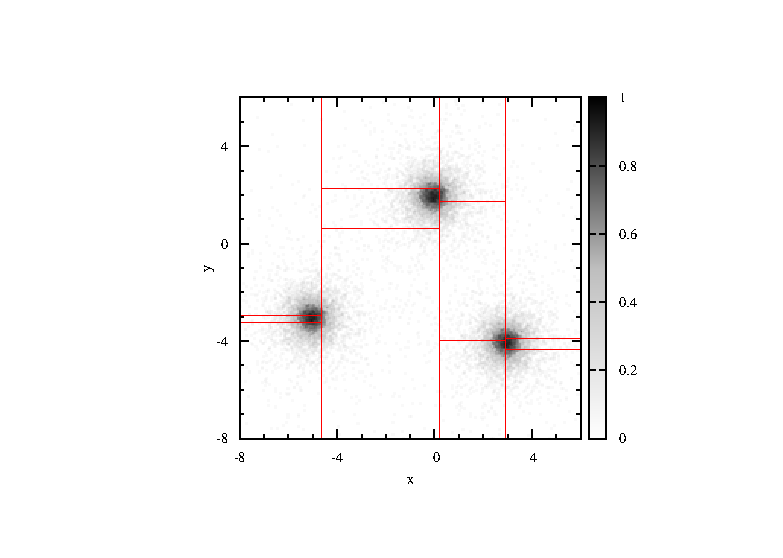
\includegraphics[width=8cm]{fig/pm3d.eps}
  \end{center}
  \caption{Example of the domain decomposition. The division is $7
    \times 6$ in 2-dimension.}
  \label{fig:decomposition}
\end{figure}

In the following, we describe how the calculation of the geometry of
subdomains (we denote this part as ``domain decomposition'') and the
exchange of particles are implemented in FDPS.  They correspond to the
member function \texttt{decomposeDomainAll} of class \texttt{DomainInfo} and
\texttt{exchangeParticle} of class \texttt{ParticleSystem}.

We adopts the ``sampling
method'' \cite{Blackston:1997:HPE:509593.509597} for the domain
decomposition, which consists of the following steps:
\begin{enumerate} 
\item Each process samples particles randomly from its own
  particles. In order to achieve the optimal load balance, the
  sampling rate of particles is changed so that it is proportional to
  the CPU time per particle spent on that
  process \cite{ishiyama:greem}. FDPS provides several options
  including this optimal balance. \label{proc:sampling}
%%
\item Each process sends their sample particles to the process with
  rank 0. Hereafter, we call this process ``root
  process''. \label{proc:gathering}
%%
\item The root process determines the new candidate subdomains  by
applying  the following procedure to x, y, and z coordinates.
 \label{proc:sorting}
%%
  \begin{itemize}
%%
  \item Sorts the sampled particles in the domain (or subdomains
    created in the previous steps) using 
    their coordinates used in the current step, 
    and divide particles into 
    $n_k$ subsets ($k$ is the coordinate axis for the current step).
    with equal number of sample particles.
  \end{itemize}
%%
\item The root process determines the final subdomains by applying the
    weighted average between the previous one and the new candidate. This
    procedure is used to stabilize the decomposition and suppress
    unnecessary oscillation. \label{proc:moving}
%%
\item The root process broadcasts the geometries of the final
    subdomains  to
  all the other processes. \label{proc:broadcasting}
%%
\end{enumerate}

The advantage of the sampling method is in its low calculation and
communication cost. They are $\mathcal{O}(N_\mathrm{s} \log
N_\mathrm{s})$ and $\mathcal{O}(N_\mathrm{s} )$, where $N_\mathrm{s}$
is the total number of sampled particles. Thus, as far as
$N_\mathrm{s}$ is not much larger than $N/n$, the average number of
particles per process, the cost of domain decomposition is negligible.

After the domain decomposition is done and the result is broadcasted
to all processes, they exchange particles so that each of them has the
particles in its domain. Since each process has the complete
information of the domain decomposition, this part is pretty
straightforward to implement. Each process looks at each of its
particles, and determines if that particle is still in its domain.  If
not, the process determines to which process that particle should be
sent. After the destinations of all particles are determined, each
process sends them out, using \texttt{MPI\_Alltoallv} function.

% LocalWords:  FDPS subdomain MPI multi subdomains DomainInfo ParticleSystem
% LocalWords:  decomposeDomainAll exchangeParticle substeps scalability
% LocalWords:  broadcasted Alltoallv


\subsection{Interaction calculation}
\label{sec:calculation}

In this section, we describe the implementation of the calculation of
interactions in FDPS. Conceptually, it consists of the following two
steps. In the first step, each process determines, for each of other
processes, which of its particles and superparticles are required by
that process for interaction calculation, and sends them to it. In the
second step, each process calculates the interactions onto
$i$-particles by calling user-defined function objects.

\if 0
\begin{enumerate}
\item Each process determines, for each of other processes, which of
  its particles and   superparticles are required by that process for
  interaction calculation,   and sends them to it.

%%
\item Each process calculates the interactions onto  $i$-particles by
  calling user-defined function objects.
\end{enumerate}
\fi

\begin{figure}
  \begin{center}
    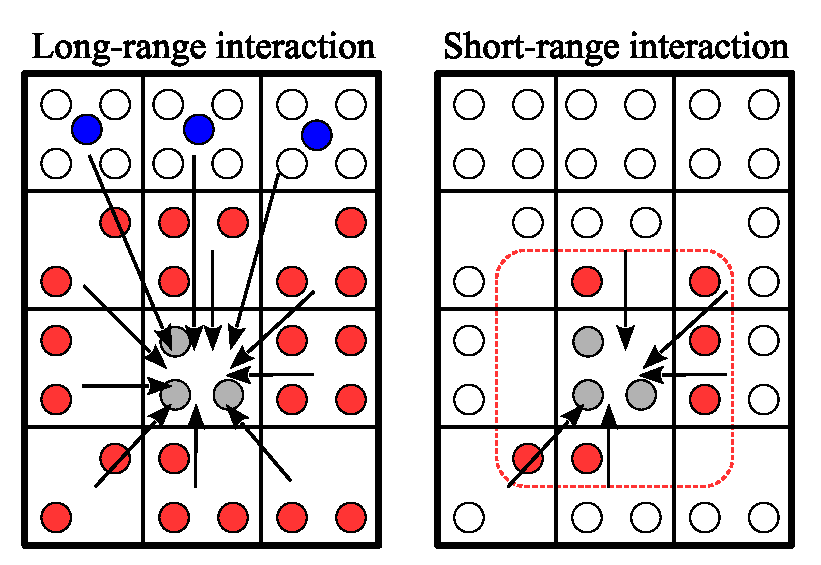
\includegraphics[width=8cm]{fig/exchangeLET.eps}
  \end{center}
  \caption{Illustration of communication among processes during the
    interaction calculation.}
  \label{fig:exchangeLET}
\end{figure}

For both steps, the octree structure is used, both for long- and
short-range interactions.
%%In step 1, 
In the first step, each process constructs the tree structure for its
local particles, and uses it to determine what data should be sent to
other processes. For the long-range interactions, this part is done
through the usual tree traversal \cite{1986Natur.324..446B,
  1990JCoPh..87..161B}. For the short-range interactions, tree
traversal is also used. A cube in a tree need to be subdivided if it
is within the cutoff length from anywhere in the domain of the process
to which the data will be sent.  The current implementation of FDPS
can handle four different types of the cutoff length for the
``short-range'' interaction: fixed, $j$-dependent, $i$-dependent and
symmetric.  For $i$-dependent and symmetric cutoffs, FDPS does the
tree traversal twice.  Figure~\ref{fig:exchangeLET} illustrates what
data are sent, for both long- and short-range interactions.

After a process receives all data it requires, it reconstructs the
tree structure which contains all information necessary to calculate
interactions on its particles.

The interaction calculation is performed using this new tree. The
procedure is the same as described in detail in the literature
\cite{1990JCoPh..87..161B, 1991PASJ...43..859M}, except for the
following two differences.  First, this part is fully multithreaded
using OpenMP, to achieve very good parallel performance. Second, for
the interaction calculation the user-provided functions are used, to
achieve the flexibility and high performance at the same time.

% LocalWords:  FDPS TreeForForceLong TreeForForceShort calcForceAllAndWriteBack
% LocalWords:  subdomains substeps octree multipole superparticles nd OpenMP
% LocalWords:  substep multithreading multithreaded


\section{Performance}
\label{sec:performance}

In this section, we report the performance of two astrophysical
applications of FDPS: a gravitational $N$-body simulation code in
section~\ref{sec:nbody} and an SPH simulation code with self-gravity
in \ref{sec:sph}.


\subsection{\secit{N}-body simulation}
\label{sec:nbody}

In this section, we discuss the performance and scalability of a
gravitational $N$-body simulation code implemented using FDPS. The
code is essentially the same as the sample code described in
section~\ref{sec:samplecode}, except for the following two differences
in the user code for the calculation of the interaction. First, here,
we used the expansion up to quadrupole moment, instead of
monopole-only one used in the sample code, to improve the
accuracy. Second, we used highly-optimized kernel developed using SIMD
builtin functions, instead of the simple one in the sample code.

We apply this code for the simulation of the Milky Way-like galaxy,
which consists of a bulge, disk, and dark matter halo.  For the review
of dynamics within galaxies, see
\cite{2014PASA...31...35D}. For examples of recent large-scale
simulations, see \cite{2011ApJ...730..109F, Bedorf:2014:PGT:2683593.2683600}.

The initial condition is the Milky Way model, the same as that
in \cite{Bedorf:2014:PGT:2683593.2683600}, consisting of a bulge,
disk, and dark matter halo.  The mass of the bulge is $4.6 \times 10^9
M_\odot$ (solar mass), and it has a spherically-symmetric density
profile of a Hernquist density profile \cite{1990ApJ...356..359H} with
the half-mass radius of $0.5$~kpc. The disk is an axisymmetric
exponential disk with the scale radius of $3$~kpc, scale height of
$200$~pc and mass $5.0 \times 10^{10}M_\odot$. The dark halo has an
Navarro-Frenk-White (NFW) density profile \cite{1996ApJ...462..563N}
with the half-mass radius of $40$~kpc and mass of $6.0 \times 10^{11}
M_\odot$. In order to realize the Milky Way model, we actually use
GalacticICS \cite{2005ApJ...631..838W}.
We also show the result for the Plummer
model \cite{1911MNRAS..71..460P}. 

\begin{figure}
  \begin{center}
    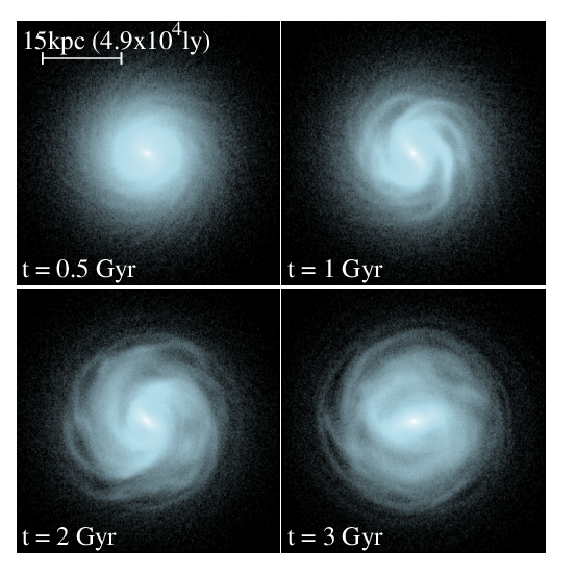
\includegraphics[width=8cm]{fig/disk.eps}
  \end{center}
  \caption{Face-on surface density maps of the bulge and disk. The
  total number of particles is $0.97$ billions. }
  \label{fig:evolutiondisk}
\end{figure}

We adopt $\theta=0.4$ for the opening angle for the tree algorithm. In
this paper, we present the weak-scaling performance of the code with
FDPS. Therefore we fixed the number of particles per node to $2.1$
million and measured the performance for number of nodes in the range
of 128 to 16384.  For the Plummer model, performance measurement for up
to $76544$ has been finished at the time of writing. The obtained
performance numbers are quite similar for these two models.

Figure~\ref{fig:evolutiondisk} illustrates the time evolution of the
bulge and disk in the run with $512$ nodes. The disk is initially
axisymmetric.  We can see that spiral structure develops (0.5 and 1
Gyrs) and central bar structure follows the spiral (1Gyrs and
later). As the bar grows, the two-arm structure becomes more visible
(3Gyrs).

Figure~\ref{fig:benchdisk} shows the measured performance. We can see
the measured efficiency and scalability are both very good. Efficiency
is very close to 50\%, for both models and for the entire range of
nodes. Wallclock time shows slight  increase for larger number of nodes,
but this is due to the increase of the calculation cost and not due to
the degradation of the efficiency. 

B\'edorf \textit{et al.}\cite{Bedorf:2014:PGT:2683593.2683600}
reported the wallclock time of 4 seconds for their 27-billion particle
simulation on the Titan system with 2048 NVIDIA Tesla K20X, with the
theoretical peak performance of 8PF (single precision, since single
precision us used for interaction calculation). This corresponds to
0.8 billion particles per second per petaflops. Our code on K computer
requires 15 seconds on 16384 nodes (2PF theoretical peak), resulting in
1 billion particles per second per petaflops. Therefore, we can
conclude that our FDPS code achieved the performance slightly better
than one of the best codes specialized to gravitational $N$-body
problem.

\begin{figure}
  \begin{center}
    \includegraphics[width=8cm]{fig/bench.eps}
  \end{center}
  \caption{Performance measured in the speed of the floating-point
    operation (top) and wallclock time per one timestep (bottom)
    plotted as functions of the number of nodes. In the bottom panel,
    time spent for interaction calculation (IC), and domain
    decomposition plus exchange particles (DD+EP) are also shown.  In
    both panels, circles and crosses indicate the Milky Way (MW)
    and Plummer (PL) models.
    }
  \label{fig:benchdisk}
\end{figure}

% LocalWords:  FDPS superparticle monopole quadrupole SIMD builtin Hernquist IC
% LocalWords:  Frenk NFW EP scalability TPP PFLOPS NVIDIA kpc axisymmetric pc
% LocalWords:  GalacticICS Gyrs timestep edorf et al petaflops Wallclock
% LocalWords:  wallclock


\subsection{SPH simulation}
\label{sec:sph}

In this section, we discuss the performance of an SPH simulation code
with self-gravity implemented using FDPS. The test problem used is the
simulation of Giant Impact (GI). The giant impact
hypothesis \cite{1975Icar...24..504H, 1976LPI.....7..120C} is one of
the most popular scenarios for the formation of the Moon. The
hypothesis is as follows. About 5 billion years ago, a Mars-sized
object (hereafter, the impactor) collided with the proto-Earth
(hereafter, the target). The collision scattered a large amount of
debris, which first formed the debris disk and eventually the
Moon. Many researchers have performed simulations of GI, using the SPH
method.
\cite{1986Icar...66..515B, 2013Icar..222..200C, 2014NatGe...7..564A}.

For the gravity, we used monopole-only kernel with $\theta=0.5$. We
adopt the standard SPH scheme
\cite{1992ARA&A..30..543M, 2009NewAR..53...78R, 2010ARA&A..48..391S}
for the hydro part. Artificial viscosity was used to handle shock waves
\cite{1997JCoPh.136..298M}, and 
the standard Balsara switch was used to reduce the shear viscosity
\cite{1995JCoPh.121..357B}. Assuming that the target and impactor
consist of granite, we adopt the equation of state of
granite \cite{1986Icar...66..515B} for the particles. The initial
conditions, such as the orbital parameters of the two objects, are the
same as those in \cite{1986Icar...66..515B}. In this paper, we report
the weak scaling performance with about 250k particles per node. For
the largest calculation, we used $1.0$ billion particles and $4096$
nodes.

Similarly to our $N$-body simulation code, we run our SPH simulation
code on K computer and Cray XC30. The maximum numbers of cores we used
are $32768$ cores ($4096$ nodes) on K computer, and $2064$ cores ($86$
nodes) on Cray XC30.

For gravity calculations, we used highly-optimized kernel developed
using SIMD builtin functions on both platforms. However, for fluid
calculations, we used the optimized kernel on the K computer, but do
not on Cray XC30.

\begin{figure}
  \begin{center}
%    \includegraphics[width=8cm]{fig/GI.eps}
    \includegraphics[width=7cm]{fig/GI.eps}
  \end{center}
  \caption{Temperature maps of the target and impactor in the run of
  $9.9$ million particles at four different epochs. }
  \label{fig:evolutionGI}
\end{figure}

Figure~\ref{fig:evolutionGI} shows the time evolution of the target
and impactor for a run with 9.9 million particles. We can see that the
shock waves are formed just after the moment of impact in both the
target and impactor (t=2050sec). The shock propagates in the target,
while the impactor is completely disrupted (t=2847sec) and debris is
ejected. Part of the debris falls back to the target, while the rest
will eventually form the disk and the Moon. So far, the resolution
used in the published papers have been much lower. We plan to use this
code to improve the accuracy of the GI simulations.

Filled and open squares in Figure~\ref{fig:benchdisk} show the
measured performance of our SPH simulation code. We can see the
measured efficiency and scalability are both very good on both
platforms, similarly to our $N$-body simulation code in the previous
section. On the K computer, efficiency is very close to 40\% for the
entire range of the number of nodes. The difference of SPH performance
between K computer and Cray XC30 is smaller than that of $N$-body
performance. This is because our SPH simulation code on Cray XC30 does
not efficiently utilize SIMD instructions for fluid
calculations. Although the SIMD instructions are used for gravity
calculations, the calculation cost is dominated by fluid calculations.

The largest number of particles used for GI simulations so far
reported is 100 million \cite{2014LPI....45.2703T}. Unfortunately,
performance numbers are not given. After we replace the interaction
kernels with SIMD-optimized ones for hydrodynamics part, we believe we
can achieve the performance not so much lower than that we achieved
for pure gravity calculation.

% LocalWords:  SPH FDPS impactor proto Balsara rr rrr Grav Wendland SIMD

% LocalWords:  builtin Wallclock timestep wallclock monopole


\section{Conclusion}
\label{sec:conclusion}

We have developed a novel framework for particle-based simulations,
FDPS.  Users of FDPS need not care about complex implementations of
domain decomposition, exchange of particles, communication of data for
the interaction calculation, or optimization for multi-core
processors.  Using FDPS, particle simulation codes which achieve high
performance and high scalability on massively parallel
distributed-memory machines can be easily developed for a variety of
problems.  As we have shown in section~\ref{sec:samplecode}, a
parallel $N$-body simulation code can be written in less than 120
lines.  Example implementations of gravitational $N$-body simulation
and SPH simulation showed excellent scalability and performance. We
hope FDPS will help researchers to concentrate on their research, by
removing the burden of complex code development for parallization and
architecture-dependent tuning.


% LocalWords:  FDPS multi SPH parallization scalability


%FDPS, \textit{FDPS}, \textbf{FDPS}, \texttt{FDPS}
%\section{Section \secit{Section}}
%\subsection{Subsection \subsecit{Subsection}}
%\subsubsection{Subsubsection}
%\paragraph{Paragraph}
%\paragraph*{Paragraph*}
%$c_\mathrm{s}$, $c_{\mathrm{s},i}$

\section{Acknowledgments}

We thank M. Fujii for providing initial conditions of spiral
simulations, T. Ishiyama for providing his Particle Mesh code, and
Y. Maruyama for being the first user of FDPS.  We are grateful to
M. Tsubouchi for her help in managing the FDPS development team. This
research used computational resources of the K computer provided by
the RIKEN Advanced Institute for Computational Science through the
HPCI System Research project (Project ID:ra000008).

\bibliographystyle{abbrv}
\bibliography{sc15_fdps}

\end{document}

% LocalWords:  FDPS Masaki Iwasawa RIKEN Minatojima minami machi Chuo ku Hyogo
% LocalWords:  Ataru Tanikawa Natsuki Hosono Keigo Nitadori Takayuki Muranushi
% LocalWords:  Junichiro Makino parallelization scalability meshfree multi SIMD
% LocalWords:  Github GreeM SPH APIs du dt sc fdps Fujii Ishiyama Maruyama HPCI
% LocalWords:  Tsubouchi ra
